\documentclass[iop]{emulateapj}

\usepackage{tikz}
\usepackage{natbib}
\usepackage{amsmath}

\usetikzlibrary{shapes.geometric, arrows}
\usetikzlibrary{fit}

\tikzstyle{hyper} = [circle, text centered, draw=black]
\tikzstyle{param} = [circle, text centered, draw=black]
\tikzstyle{data} = [circle, text centered, draw=black, line width=2pt]
\tikzstyle{arrow} = [thick,->,>=stealth]

\newcommand{\myemail}{aimalz@nyu.edu}
\newcommand{\textul}{\underline}
\newcommand{\chippr}{\texttt{CHIPPR} }

\shorttitle{How to obtain the redshift distribution from probabilistic redshift 
estimates}
\shortauthors{Malz, et al.}

\begin{document}

\title{How to obtain the redshift distribution from probabilistic redshift 
estimates}

\author{Alex Malz\altaffilmark{1}, David W. Hogg\altaffilmark{1,2,3,4}, Phil 
Marshall\altaffilmark{5}, \& Others}
\email{aimalz@nyu.edu}

\altaffiltext{1}{Center for Cosmology and Particle Physics, Department of 
Physics,
  New York University, 726 Broadway, 9th floor, New York, NY 10003, USA}
\altaffiltext{2}{Simons Center for Computational Astrophysics, 162 Fifth 
Avenue, 7th floor, New York, NY 10010, USA}
\altaffiltext{3}{Center for Data Science, New York University, 60 Fifth Avenue, 
7th floor, New York, NY 10003, USA}
\altaffiltext{4}{Max-Planck-Institut f\"ur Astronomie, K\"onigstuhl 17, D-69117 
Heidelberg, Germany}
\altaffiltext{5}{[SLAC]}

\begin{abstract}
The redshift distribution $n(z)$ is a crucial ingredient for weak lensing 
cosmology.  Spectroscopically confirmed redshifts for the dim and numerous 
galaxies observed by weak lensing surveys are expected to be inaccessible, 
making photometric redshifts (photo-$z$s) the next best alternative.  Because 
of the nontrivial inference involved in their determination, photo-$z$ point 
estimates are being superseded by photo-$z$ probability distribution functions 
(PDFs).  However, analytic methods for utilizing these new data products in 
cosmological inference are still evolving.  This paper presents a novel 
approach to estimating the posterior distribution over $n(z)$ from a survey of 
galaxy photo-$z$ PDFs based upon a probabilistic graphical model of 
hierarchical inference.  We present the Cosmological Hierarchical Inference 
with Probabilistic Photometric Redshifts (\chippr) code implementing this 
technique, as well as its validation on mock data and testing on the 
\texttt{Buzzard} simulations.  \chippr yields a more accurate characterization 
of $n(z)$ containing information beyond the best-fit estimator produced by 
traditional procedures.  The publicly available code is easily extensible to 
other one-point statistics that depend on redshift.

\end{abstract}

\keywords{catalogs --- cosmology: cosmological parameters --- galaxies: 
statistics --- gravitational lensing: weak --- methods: analytical --- methods: 
data analysis --- methods: statistical --- techniques: photometric}

\section{Introduction}
\label{sec:introduction}

After a brief literature review addressing how photo-$z$ PDFs are currently 
used in cosmology, this paper aims to answer the following questions:

\begin{itemize}
	\item Why should we question existing methods?
	\item How can we improve the effectiveness of using photo-$z$ PDFs in 
inference?
	\item How does the result of \chippr compare to established estimators 
in terms of the accuracy of $n(z)$?
	\item How significant is the effect of the discrepancy between $n(z)$ 
estimators on cosmological constraints?
\end{itemize}

\section{Method}
\label{sec:method}

This paper presents a mathematically consistent method for obtaining the 
posterior distribution over the redshift density function $n(z)$ using a 
catalog of photo-$z$ PDFs.

\subsection{Model}
\label{sec:model}

The directed acyclic graph of Fig. \ref{fig:pgm} represents a probabilistic 
graphical model for hierarchical inference of $n(z)$, the mathematical 
interpretation of which will be presented below.

\begin{figure}
	\begin{center}
		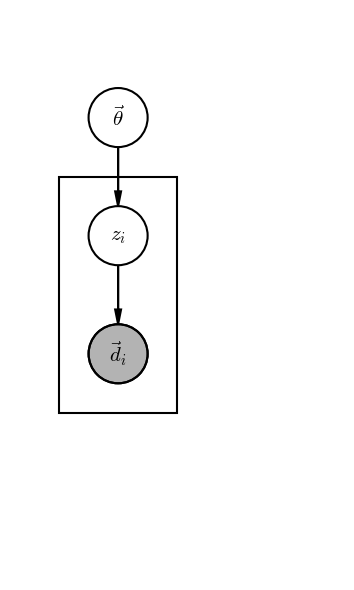
\includegraphics[width=0.5\textwidth]{pgm.png}
		\caption{\textbf{Replace \texttt{daft} version with more 
polished \texttt{tikz} version.}}
	\label{fig:pgm}
	\end{center}
\end{figure}

\textbf{Math from \texttt{prob-z} version will go here.}

This framework entails a number of choices and assumptions that must be 
addressed explicitly.

\begin{enumerate}
	\item While we advocate for the approach of hierarchical inference, the 
probabilistic graphical model presented here is not the only one that could be 
proposed.
\end{enumerate}

\subsection{Alternative Approaches}
\label{sec:others}

It is useful to translate some popular existing methods for deriving $n(z)$ 
from photo-$z$ PDFs into the mathematical framework of Sec. \ref{sec:model}.

\subsection{Implementation}
\label{sec:implementation}

The publicly available \chippr code implements the probabilistic graphical 
model presented in Sec. \ref{sec:model}.  

In addition to the choices and assumptions underlying the probabilistic 
graphical model, the implementation of \chippr makes choices and assumptions of 
its own.

\begin{enumerate}
	\item \chippr currently only accepts photo-$z$ PDFs and produces $n(z)$ 
samples of a single format, that of the piecewise constant parametrization, 
also referred to as a binned histogram parametrization and a sum of top hat 
functions.
\end{enumerate}

\section{Validation on Simple Mock Data}
\label{sec:validation}

The superiority of \chippr over alternative approaches is demonstrated in a 
number of compelling test cases on mock data.  Each experiment is characterized 
by a single change to a fiducial case in order to isolate the influence of 
systematic effects known to be relevant to photo-$z$ estimation and propagation 
in analysis.  

\subsection{Mock Data \& Metrics}
\label{sec:validintro}

The mock data in these tests consists of photo-$z$ interim posteriors rather 
than photometric data because the various existing methods for deriving 
photo-$z$ interim posteriors do not in general yield results that are 
consistent with one another, indicating that their systematics are not 
well-understood.  Because the mock data is independent of any choice of 
photo-$z$ PDF production method, we not only ensure that our photo-$z$ interim 
priors are perfectly understood but also deter readers from assuming that 
\chippr has any preference over the method by which photo-$z$ interim 
posteriors are derived from photometric data.

\subsubsection{Mock Data}
\label{sec:mockdata}

The mock data used here are produced by the following steps.  This method for 
deriving mock data is referred to as the fiducial case, and variations on it 
will refer directly to the steps that are altered.

\subsubsection{$n(z)$ Accuracy Metric}
\label{sec:accuracy}

The Kullback-Leibler divergence will be used as the primary measure of the 
accuracy of estimators of $n(z)$ in cases of mock data with known true 
redshifts.

\textbf{Review precision and bias from \texttt{kld.ipynb} and interpret in 
terms of a \% difference.}

\subsection{Emulated Data Quality Effects}
\label{sec:likelihoods}

In the following test cases, the properties of the mock photo-$z$ likelihoods 
are varied in an effort to emulate known systematics in photo-$z$ estimation.

\subsubsection{Intrinsic Scatter}
\label{sec:intscat}

One major concern about photo-$z$s is the intrinsic scatter of point 
estimators, including those derived from photo-$z$ PDFs, that is observed to 
varying extents with every existing photo-$z$ algorithm and illustrated in Fig. 
\ref{fig:intscat}.  

\begin{figure}
	\begin{center}
		%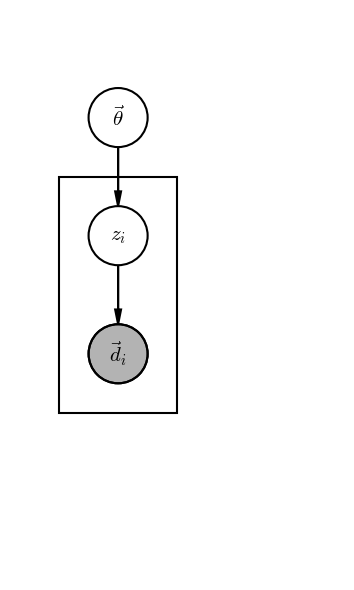
\includegraphics[width=0.5\textwidth]{pgm.png}
		\caption{[plot of $z_{phot}$ vs. $z_{spec}$ with varying 
intrinsic scatter]}
		\label{fig:intscat}
	\end{center}
\end{figure}

To emulate intrinsic scatter, we modify the fiducial case to simply broaden the 
single Gaussian component of the likelihood.  To enforce self-consistency, the 
mean is drawn from a Gaussian distribution with the newly increased variance.

\subsubsection{Template-like Catastrophic Outliers}
\label{sec:tempcatout}

In addition to intrinsic scatter, photo-$z$ methods employing template fitting 
tend to produce catastrophic outliers that are distributed to be broad in 
$z_{spec}$ and narrow in $z_{phot}$, as in Fig. \ref{fig:tempfail}.  The 
systematic behind these catastrophic outliers may be described as an attractor 
in the space of $z_{phot}$; some galaxies at a range of $z_{spec}$ map onto a 
single $z_{phot}$ (with some scatter) if their true SED does not have 
sufficiently strong features (as is the case for blue galaxies), leading 
galaxies of that type at many $z_{spec}$ to have similar colors.

\begin{figure}
	\begin{center}
		%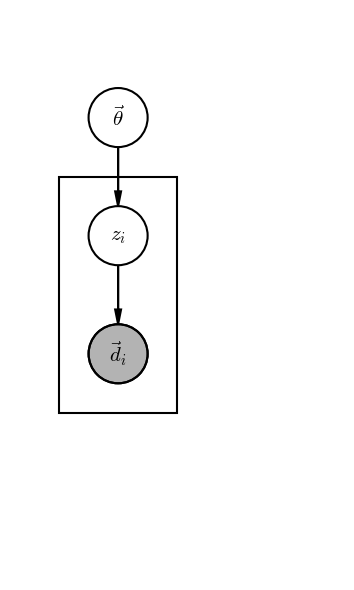
\includegraphics[width=0.5\textwidth]{pgm.png}
		\caption{[plot of $z_{phot}$ vs. $z_{spec}$ with template-like 
catastrophic outliers]}
		\label{fig:tempcatout}
	\end{center}
\end{figure}

\subsubsection{Training-like Catastrophic Outliers}
\label{sec:traincatout}

Data driven photo-$z$ methods tend to suffer from a different form of 
catastrophic outliers that are distributed to be narrow in $z_{spec}$ and broad 
in $z_{phot}$, as in Fig. \ref{fig:trainfail}.  The systematic behind these 
catastrophic outliers may be described as an attractor in the space of 
$z_{spec}$; some galaxies near a particular $z_{spec}$ map to a range of 
$z_{phot}$ if their true SED's features fall between photometric filters, 
leading to many galaxies near that $z_{spec}$ to have similar colors.

\begin{figure}
	\begin{center}
		%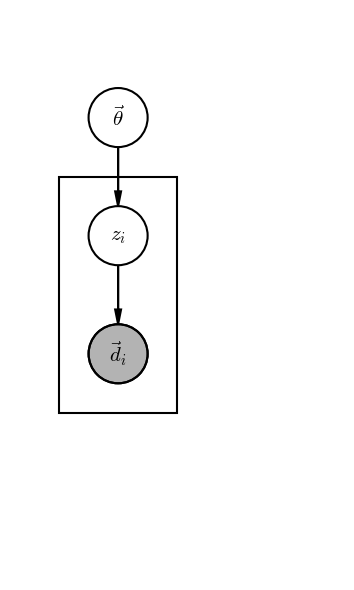
\includegraphics[width=0.5\textwidth]{pgm.png}
		\caption{[plot of $z_{phot}$ vs. $z_{spec}$ with training-like 
catastrophic outliers]}
		\label{fig:traincatout}
	\end{center}
\end{figure}

\subsection{Emulated Interim Prior Effects}
\label{sec:priors}

The interim prior encapsulates the information about the relationship between 
observed photometry and redshift upon which a photo-$z$ estimate is based.  
Interim priors are in general not identical to the true $n(z)$ we wish to 
estimate; if they were, we would not need any data!  For template fitting 
photo-$z$ methods, the interim prior is usually an input chosen by the 
researcher.  However, for many machine learning methods, the interim prior is 
some function of the training set data that may be influenced by random numbers 
and is rarely output with the redshift estimates.  Interim priors for template 
fitting methods tend to have incomplete coverage in the space of true 
photometry, because they are limited by the choice of the library of SEDs.  
Interim priors for machine learning methods tend to have incomplete coverage in 
the space of redshifts, because there are fewer galaxies with spectroscopically 
confirmed redshifts at high redshifts than low redshifts.

Existing $n(z)$ estimation routines will always produce a biased estimator when 
the interim prior is not equal to the true $n(z)$.  We demonstrate here that 
regardless of the appropriateness of the interim prior as an approximation to 
the true $n(z)$, \chippr is not affected by the choice of the interim prior so 
long as it has nontrivial coverage.

\subsubsection{Template-like Interim Prior}
\label{sec:tempintpr}

An interim prior based on a template library may be a sum of smooth functions 
representing $n(z)$ for each SED type in the library.  Template libraries do 
not include every possible galaxy SED, and the $n(z)$ used for each SED type 
may not be accurate.  The interim prior shown in Fig. \ref{fig:tempintpr} is an 
emulation of an interim prior corresponding to a template library of this type.

\begin{figure}
	\begin{center}
		%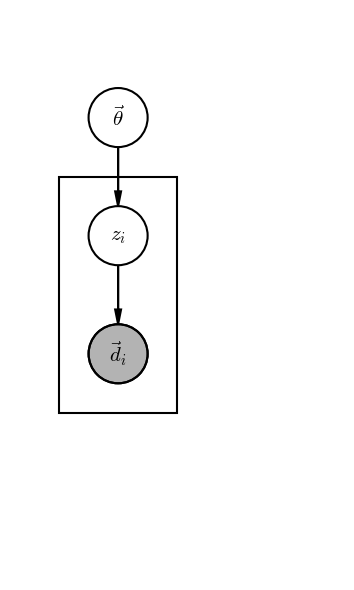
\includegraphics[width=0.5\textwidth]{pgm.png}
		\caption{[plot of template-like interim prior]}
		\label{fig:tempintpr}
	\end{center}
\end{figure}

\subsubsection{Training-like Interim Prior}
\label{sec:trainintpr}

An interim prior based on a training set may be biased toward low redshifts due 
to the dearth of distant galaxies with spectroscopic redshifts.  The interim 
prior shown in Fig. \ref{fig:trainintpr} is an emulation of an interim prior 
corresponding to a training set biased in this way.

\begin{figure}
	\begin{center}
		%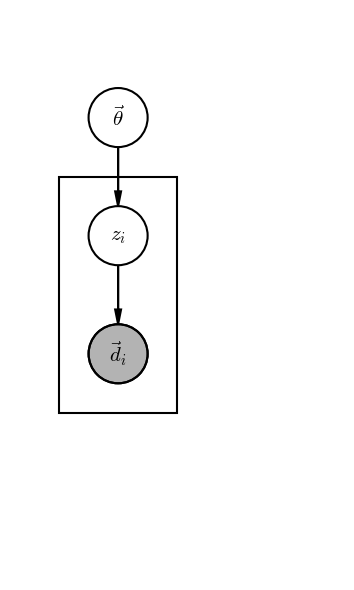
\includegraphics[width=0.5\textwidth]{pgm.png}
		\caption{[plot of training-like interim prior]}
		\label{fig:trainintpr}
	\end{center}
\end{figure}

\subsection{Underlying $n(z)$ Effects}
\label{sec:truth}

Existing $n(z)$ estimators are systematically smoother than the true $n(z)$.  
Here we show that the traditional estimators of $n(z)$ cannot recover a highly 
featured $n(z)$.  The implication of this failure is quite serious; the 
consistently smooth, unimodal $n(z)$ estimates appearing in the literature 
could result from much more featured true redshift distributions, and there 
would be no way to catch this error without using a fully probabilistic method.

\subsubsection{Featured $n(z)$}
\label{sec:featured}

In this test, we choose the true $n(z)$ of Fig. \ref{fig:featured}, which has 
nontrivial structure.

\begin{figure}
	\begin{center}
		%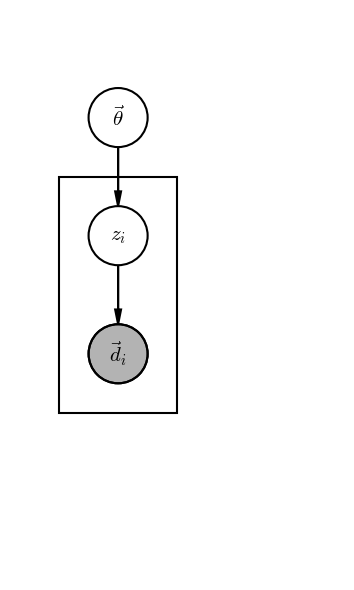
\includegraphics[width=0.5\textwidth]{pgm.png}
		\caption{[plot of a highly featured true $n(z)$]}
		\label{fig:featured}
	\end{center}
\end{figure}

\section{Application to Realistic Mock Data}
\label{sec:application}

To show how the choice of $n(z)$ estimator propagates to cosmological 
constraints, we apply \chippr to a data from a realistic cosmological 
simulation (probably \texttt{Buzzard}).

\subsection{Mock Data \& Metrics}
\label{sec:appintro}

As in Sec. \ref{sec:validintro}, the mock data takes the form of photo-$z$ 
interim posteriors, but that is where the similarity ends.  These photo-$z$ 
interim posteriors are derived from the photometry resulting from the 
\texttt{Buzzard} simulation by way of [method used to make the interim 
posteriors].  Because the simulation begins with setting true values of the 
cosmological parameters, the different estimators of $n(z)$ are propagated 
through a forecasting code to produce error ellipses on the cosmological 
parameters.

\subsubsection{Mock Data}
\label{sec:buzzard}

The details of the \texttt{Buzzard} simulation will be summarized here.

\subsubsection{Cosmological Constraint Metric}
\label{sec:cosmo}

Because the mock data is associated with true values of the cosmological 
parameters, we may compare the quality of cosmological constraints.

\textbf{Check Dark Energy Task Force metrics on error ellipses, 
multi-dimensional KLD, centroid offset, etc.}

\subsection{Results}
\label{sec:results}

\begin{figure}
	\begin{center}
		%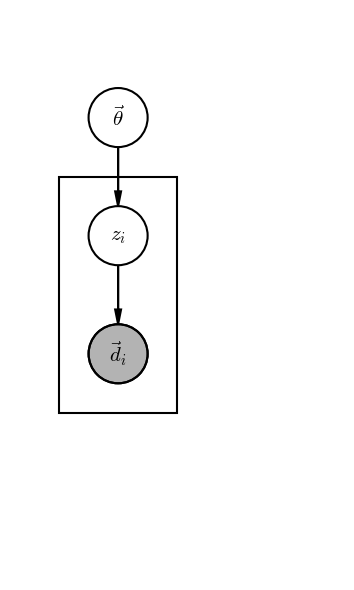
\includegraphics[width=0.5\textwidth]{pgm.png}
		\caption{[moneyplot]}
		\label{fig:money}
	\end{center}
\end{figure}

\section{Discussion}
\label{sec:discussion}

Thee results of Fig \ref{fig:money} have significant implications for the 
developing data analysis pipelines of next-generation telescope surveys.  
However, the method presented here has its own limitations, which are 
reiterated to discourage the community from applying our work inappropriately.

There are a number of extensions of the work presented in this paper that will 
be pursued in future work.

\section{Conclusion}
\label{sec:conclusion}

We now summarize answers to the questions posed in the introduction:

\begin{itemize}
	\item Existing $n(z)$ estimation methods produce biased estimators that 
propagate to inaccuracies in characterizing the cosmological parameters.
	\item Photo-$z$ PDFs are probabilistic data products so must be handled 
in a mathematically consistent manner such as the probabilistic graphical model 
outlined in this paper.
	\item In addition to coming with its own error distribution, the $n(z)$ 
estimator produced by \chippr is quantifiably more accurate than established 
estimators.
	\item Propagation of the \chippr result leads to a quantifiable 
improvement in the constraints on cosmological parameters.
\end{itemize}

In conclusion, we discourage the community from continuing to use the stacked 
estimator and reductions of photo-$z$ PDFs to redshift point estimates in 
obtaining estimators of $n(z)$.  \chippr is freely available to the community 
for incorporation into evolving data analysis pipelines.  



\begin{acknowledgements}
AIM thanks Mohammadjavad Vakili for insightful input on statistics, Geoffrey 
Ryan for assistance in debugging, and Boris Leistedt for helpful comments 
provided in the preparation of this paper.
\end{acknowledgements}


\end{document}
